\chapter{Game AI}
%Babbage, Charles -- . . .every game of skill is susceptible of being played by an automaton.
%Minsky, Marvin -- It is not that the games and mathematical problems are chosen because they are clear and simple; rather it is that they give us, for the smallest initial structures, the greatest complexity, so that one can engage some really formidable situations after a relatively minimal diversion into programming. From Semantic Information Processing, p. 12. Cambridge, MA: MIT Press (1968).
% If you'd like to know, I can tell you that in your universe you move freely in three dimensions that you call space. You move in a straight line in a fourth, which you call time, and stay rooted to one place in a fifth, which is the first fundamental of probability. After that it gets a bit complicated, and there's all sort of stuff going on in dimensions thirteen to twenty-two that you really wouldn't want to know about. All you really need to know for the moment is that the universe is a lot more complicated than you might think, even if you start from a position of thinking it's pretty damn complicated in the first place. I can easily not say words like "damn" if it offends you. H2G2

%%% Some characteristics of Game AI
%%% high-level perception, commonsense reasoning, NLP, speech processing,
%%% gesture processing, planning \& counterplanning, cognitive modeling,
%%% plan recognition, soft real-time response, reactive behavior, teamwork,
%%% scheduling, path planning, spatial reasoning, temporal reasoning,
%%% opponent modeling, learning, knowledge acquisition

\begin{verse}\textit{
\\
David: What is the primary goal?\\
Joshua: You should know, Professor. You programmed me.\\
David: Oh, come on. What is the primary goal?\\
Joshua: To win the game.\\
} Wargames (1983)\end{verse}
%\lettrine[image=true, lines=3, findent=3pt, nindent=0pt]{lettrines/O.png}{r}
\lettrine{O}{r}
 is it? ``Game AI'', simultaneously a research topic, an industry standard practice, from a staple to a part of the gameplay. Its uses range from character animation, to behavior modeling and strategic play. In this chapter, we will give our educated guess about the goals of game AI, and review what exists for a broad category of games: single player games, abstract strategy games, partial information and/or stochastic games, computer games. Let us then focus on game-play (from a player point of view) characteristics of theses games so that we can enumerate game AI needs. %%% XXX
%\lettrine[image=true, lines=3, findent=3pt, nindent=0pt]{lettrines/W.png}{hat} is game AI? What are the goals of AI in games? What are its characteristics? Why is game AI an interesting subject for research? 

%%%%%%%%%%%%%%%%%%%%%%%%%%%%%%%%%%%%%%%%%%%%%%%%%%%%%%%%%%%%%%%%%% 

\section{Goals of Game AI}
%\lettrine[lines=1, lhang=.3]{W}{hat} are the goals of game AI?
Non-playing characters (NPC, also called ``mobs'') are here to stay. Being it in ever more immersive single player adventures (The Elder Scrolls V: Skyrim), part of a cooperative gameplay (World of Warcraft, Left 4 Dead) or as helpers on our side or trainers against us (``pets'', strategy games), they are of interest for the game industry, but also for robotics, to study human cognition and for artificial intelligence in the large.

\subsection{Win}
%%%Not solved: humans are the best
During the last decade, the video games industry has seen the emergence of ``e-sport''. It is the professionalization of specific competitive games at the higher levels, as in sports: with spectators, leagues, sponsors, fans and broadcasts. A %non-exhaustive 
list of major electronic sports games includes (but is not limited to): StarCraft: Brood War, Counter-Strike, Quake III, Warcraft III, Halo, StarCraft II. The first game to have had progamers was StarCraft: Brood War, in Korea, with top players earning more than top soccer players. Top players earn more than \$400,000 a year but the professional average is below, around \$50-60,000 a year \citep{TeamLiquidPGMIncome}, against the average South Korean salary at \$16,300 in 2010. Currently, Brood War is being slowly phased out to StarCraft II (still 4.9 millions players in South Korea in 2011 \cite{CitationNeeded}). There are TV channels broadcasting Brood War (OnGameNet, previously also MBC Game) or StarCraft II (GOM TV, streaming) and for which it constitutes a major chunk of the air time. %in 2010 in South Korea, the average salary for a professional StarCraft player was \$60,000 against the average salary at \$16,300\citep{StarCraftPGM}). 
``E-sport'' is important to the subject of game AI because it ensures competitiveness of the human players. It is less challenging to write a competitive AI for game played by few and without competitions than to write an AI for Chess, Go or StarCraft. E-sport, through the distribution of ``replays'' also ensures a constant and heavy flow of human player data to mine and learn from. Finally, cognitive science researchers (like the Simon Fraser University Cognitive Science Lab) study the cognitive aspects (attention, learning, re) of high level RTS playing\cite{CitationNeeded}.

Good human players, through their ability to learn and adapt, and through high-level strategic reasoning, are still undefeated. Single players are often frustrated by the NPC behaviors in non-linear (not fully scripted) games. Nowadays, video games AI could be used part of the gameplay as a challenge to the player. 
This is not the case in most of the games though, in decreasing order of resolution of the problem\footnote{We deal in gameplay potentials here, particularly considering non-linear games, current RPG and MMORPG are often linearly limited \textit{because} of the untracted``world interacting NPC'' AI problem. Otherwise, linear RPG AI fare often better than team FPS AI.}: fast FPS (first person shooters)\newglossaryentry{FPS}{name=FPS,description={First Person Shooter: egocentric shooter game, strong sub-genres are fast FPS, also called ``Quake-likes'', e.g. Quake III; and team/tactical FPS, e.g. Counter-Strike, Team Fortress 2}}, team FPS, RPG (role playing games)\newglossaryentry{RPG}{name=RPG,description={Role Playing Game, e.g. Dungeons \& Dragons based Baldur's Gate}}, MMORPG (Massively Multi-player Online RPG)\newglossaryentry{MMORPG}{name=MMORPG,description={Massively Multi-player Online Role Playing Game, distinct of RPG by the scale of cooperation sometimes needed to achieve a common goal, e.g. Dark Age of Camelot, World of Warcraft}}, RTS (Real-Time Strategy)\newglossaryentry{RTS}{name=RTS,description={Real-Time Strategy games are (mainly) allocentric economic and military simulations from an operational tactical/strategist commander viewpoint, e.g. Command \& Conquer, Age of Empires, StarCraft, Total Annihilation}}. These games in which artificial intelligences do not beat top human players on equal footing requires increasingly more cheats to even be a challenge (not for long as they mostly do not adapt). AI cheats encompass (but are not limited to):
\begin{itemize}
\item RPG NPC often have at least 10 times more hit points (health points) than their human counterparts in equal numbers,
\item FPS bots can see through walls and use perfect aiming,
\item RTS bots see through the ``fog of war'' and have free additional resources.
\end{itemize}
How do we build game robotic players (``bots'', AI, NPC) which can provide some challenge, or be helpful without being frustrating, while staying fun?


\subsection{Fun}
%%%Not solved: humans are the most fun to play with
The main purpose of gaming is entertainment. Of course, there are subgenres of serious gaming or ``gamification'' of learning, but the majority of people playing games are having fun. Cheating AI are not fun, and so the re-playability of single player games is very low. The vast majority of games which are still played after the single player mode are multi-player games, because humans are the most fun to play with. So how do we get game AI to be fun to play with? The answer seems to be 3-fold:
\begin{itemize}
\item For competitive and PvP\newglossaryentry{PvP}{name=PvP,description={Players versus Players}}
(players versus players) games: improve game AI so that it can play well \textit{on equal footing with humans},
\item for cooperative and PvE\newglossaryentry{PvE}{name=PvE,description={Players vs Environment}}
(players vs environment) games: optimize the AI for fun, ``epic wins'': the empowerment of playing your best and just barely winning,
\item give the AI all the tools to adapt the game to the players: game directors (Left 4 Dead, Dark Spore), procedural content generation (Mario PCG).
\end{itemize}
In all cases, a good AI should be able to learn for the players' actions, recognize their behavior to deal with it in the most entertaining way. Examples for a few mainstream games: World of Warcraft instances or StarCraft II missions could be less predictable (less scripted) and always ``just hard enough'', Battlefield 3 or Call of Duty opponents could have a longer life expectancy (5 seconds in some cases), Skyrim's follower NPC could avoid blocking the player in doors, or going in front when she casts fireballs.

\subsection{Programming}
How do game developers want to deal with game AI programming? We have to understand the needs of industry game AI programmers: 
\begin{itemize}
    \item computational efficiency (particularly for real-time games with advanced graphics, the AI CPU budget is low),
    \item game designers often want to remain in control of the behaviors (and editing tools have to be usable by them),
    \item scalability (as much autonomy as possible), ``debugability'' (huge states spaces due to the presence of the player(s)), re-use accross games (game independant logic).
\end{itemize}
So, programmers can ``hard code'' the behaviors and their switches, for some structuring they have finite state machines \citep{FSM_AIGameProgWisdom2003}. This solution does not scale well (exponential increase in the number of transitions), nor do they generate autonomous behavior, and they can be cumbersome for the game designers to interact with. Hierarchical FSM \citep{CitationNeeded} is a partial answer to these problems: they scale better due to the sharing of transitions between macro-states and are more readable for game designers who can zoom-in on macro/englobing states. They still represent way too much programming work for complex behavior and are not more autonomous than classic FSM. Planning (using a search heuristic in the states space) efficiently gives autonomy to virtual characters. Planners like hierarchical task networks (HTN \citep{Erol_htnplanning}, Armed Assault, Killzone 2 \citep{ArmA1_HTN,Killzone2_HTN}) or STRIPS (\citep{FikesSTRIPS}, F.E.A.R \citep{orkinGDC_FEAR}) generate complex behaviors in the space of the combinations of specified states, and the logic can be re-used accross games. The drawbacks can be a large computational budget (for many agents and/or a complex world), the difficulty to specify reactive behavior, and less (or harder) control from the game designers. Behavior trees (Halo 2 \citep{Isla}, Spore) are a popular in-between HTN and HFSM technique providing scability through a tree-like hierarchy, control through tree editing and some autonomy through a search heuristic (for valid nodes).
A transversal technique for ease of use is to program game AI with a script (LUA, Python) or domain specific language (DSL\newglossaryentry{DSL}{name=DSL,description={Domain Specific Language}}). From a programming or design point of view, it will have the drawbacks of the models it is based on. If everything is allowed (low-level inputs and outputs directly in the DSL), everything is possible at the cost of cumbersome programming, debugging and few re-use.

Even with scalable\footnote{both computationally and in the number of lines of codes to write to produce a new behavior} architectures like behavior trees or the autonomy that planning provides, there are limitations (burdens on programmers/designers or CPU/GPU):
\begin{itemize}
    \item complex worlds require either very long description of the state (in propositional logic) or high expressivity (higher order logics) to specify well-defined behaviors,
    \item the search space of possible actions increases exponentially with the interactivity (complexity) of the world, thus requiring ever more efficient pruning techniques,
    \item once human players are in the loop (ain't that the purpose of a game?), uncertainty has to be taken into account. Previous approaches can be ``patched'' to deal with uncertainty, at what cost?
\end{itemize}
Our thesis is that we can learn complex behaviors from exploration or observations (of human players) without the need to be explicitely programmed. Furthermore, the game designers can stay in control by choosing which demonstration to learn from and tuning parameters by hand if wanted. \citet{lehy04} showed it in the case of FPS AI (Unreal Tournament), with \textit{inverse programming} to learn reactive behaviors from human demonstration. We extend it to tactical and even strategic behaviors.

%%%%%%%%%%%%%%%%%%%%%%%%%%%%%%%%%%%%%%%%%%%%%%%%%%%%%%%%%%%%%%%%%% 

\section{Single Player Games}

Single player games are not the main focus of our thesis, but they present a few interesting AI characteristics. They encompass all kinds of human cognitive abilities, from reflexes to higher level thinking.

\subsection{Action games}
%%% Mario, racing, PacMan
Platform games (Mario, Sonic), time attack racing games (TrackMania), solo shoot-them-up (``schmups'', Space Invaders, DodonPachi), sports games and rhythm games (Dance Dance Revolution, Guitar Hero) are games of reflexes, skill and level knowledge. The main components of game AI in these genres is a quick path search heuristic, often with a dynamic environment. There have been Mario \citep{TogeliusMario10}, PacMan \citep{PacManCEC11} and racing competitions \citep{CarRacingWCCI08}. The winners often use (clever) heuristics coupled with a search algorithm (A* for instance). As there are no human opponents, reinforcement learning and genetic programming works well too.

XXX

\subsection{Puzzles}
%%% Myst, Tetris, point and clicks, Patience
Point and click (Monkey Island, Kyrandia, Day of the Tentacle), graphic adventure (Myst, Heavy Rain), (tile) puzzles (Minesweeper, Tetris) games are games of logical thinking and puzzle solving. The main components of game AI in these genres is an inference engine with sufficient domain knowledge (an ontology). AI research is not particularly active in the genre of puzzle games, perhaps because solving them has more to do with writing down the ontology than with using new AI techniques. A classic well-studied logic-based, combinatorial puzzle is Sudoku, which has been formulated as a SAT-solving \citep{lynce2006sudoku} and constraint satisfaction problem \citep{Simonis2005}.

%%%%%%%%%%%%%%%%%%%%%%%%%%%%%%%%%%%%%%%%%%%%%%%%%%%%%%%%%%%%%%%%%% 

\section{Abstract Strategy Games}
%%% http://en.wikipedia.org/wiki/Game_complexity
%%% http://en.wikipedia.org/wiki/Solved_board_games
\subsection{Tic-tac-toe, Minimax}
Tic-tac-toe (noughts and crosses) is a solved game\newglossaryentry{solvedgame}{name={solved game},description={a game whose outcome can be correctly predicted from any position when each side plays optimally}}, meaning that it can be played optimally from each possible position. How did it came to get solved? Each and every possible positions (26,830) have been analyzed by a Minimax (or its variant Negamax) algorithm. Minimax is an algorithm which can be used to determine the optimal score a player can get for a move in a zero-sum game\newglossaryentry{zerosumgame}{name={zero-sum game},description={a game in which the total score of each players, from one player's point-of-view, for every possible strategies, adds up to zero; \textit{i.e.} ``a player benefits only at the expense of others''}}. The Minimax theorem states:
\begin{mythm}
For every two-person, zero-sum game with finitely many strategies, there exists a value V and a mixed strategy for each player, such that (a) Given player 2's strategy, the best payoff possible for player 1 is V, and (b) Given player 1's strategy, the best payoff possible for player 2 is -V.
\end{mythm}
Applying this theorem to Tic-tac-toe, we can say that winning is +1 point for the player and losing is -1, while draw is 0. The exhaustive search algorithm which takes this property into account in described in Algorithm~\ref{alg:minimax}. The result of applying this algorithm to the Tic-tac-toe situation of Fig.~\ref{fig:TTT} is exhaustively represented in Fig.~\ref{fig:minimaxTTT}. For zero-sum games (``strictly competitive games'' as abstract strategy games discussed here), there is a (simpler) Minimax variant called Negamax, shown in Algorithm~\ref{alg:negamax} in Appendix~\ref{apdx:gameAI}.
\begin{algorithm}
\caption{Minimax algorithm}
\label{alg:minimax}
\begin{algorithmic}
\Function{mini}{depth}
    \If{$depth \leq 0$}
        \State \Return $-value()$
    \EndIf
    \State $min \gets +\infty$
    \ForAll{possible moves}
        \State $score \gets maxi(depth-1)$
        \If{$score < min$}
            \State $min \gets score$
        \EndIf 
    \EndFor
    \State \Return $min$
\EndFunction

\Function{maxi}{depth}
    \If{$depth \leq 0$}
        \State \Return $value()$
    \EndIf
    \State $max \gets -\infty$
    \ForAll{possible moves}
        \State $score \gets mini(depth-1)$
        \If{$score > min$}
            \State $max \gets score$
        \EndIf
    \EndFor 
    \State \Return $max$
\EndFunction
\end{algorithmic}
\end{algorithm}

\begin{figure}
\begin{center}
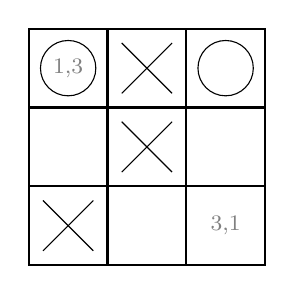
\begin{tikzpicture}
[thick]
  \foreach \x in {1,2,3}
    \foreach \y in {1,2,3}
    {
      \draw (\x,\y) +(-.5,-.5) rectangle ++(.5,.5);
    }

  \draw (1,3) node{\begin{footnotesize}\textcolor{black!50}{1,3}\end{footnotesize}};
  \draw (3,1) node{\begin{footnotesize}\textcolor{black!50}{3,1}\end{footnotesize}};

  \draw (2,3) node{\tikz \draw (-.32,-.32) -- (.32,.32);};
  \draw (2,3) node{\tikz \draw (-.32,.32) -- (.32,-.32);};

  \draw (2,2) node{\tikz \draw (-.32,-.32) -- (.32,.32);};
  \draw (2,2) node{\tikz \draw (-.32,.32) -- (.32,-.32);};

  \draw (1,1) node{\tikz \draw (-.32,-.32) -- (.32,.32);};
  \draw (1,1) node{\tikz \draw (-.32,.32) -- (.32,-.32);};

  \draw (1,3) node{\tikz \draw (0,0) circle (10pt);};

  \draw (3,3) node{\tikz \draw (0,0) circle (10pt);};
\end{tikzpicture}
\caption{A Tic-tac-toe board position, ``circles'' turn to play. The couples of numbers explain the numbering (left to right, bottom to top, starting at 1) of the grid.}
\label{fig:TTT}
\end{center}
\end{figure}

\begin{figure}
%%%\hspace{-0.8cm}
\begin{center}
\begin{tikzpicture}
    [thick,
level 1/.style={sibling distance=42mm},
level 2/.style={sibling distance=14mm},
level 3/.style={sibling distance=7mm}
]
\begin{footnotesize}
  \node[ellipse,draw] {Fig.~\ref{fig:TTT} state}
    child {node[rectangle,draw] {0}
      child {node[circle,draw] {-1}
          edge from parent node[pos=0.5,fill=black!20] {2,1}
        }
      child {node[circle,draw] {0}
          child {node[rectangle,draw] {0}
              child {node[circle,draw] {0}
                edge from parent node[pos=0.5,fill=black!20] {3,2}}
              edge from parent node[pos=0.5,left,fill=black!20] {2,1}
            }
          child {node[rectangle,draw] {0}
              child {node[circle,draw] {-1}
                edge from parent node[pos=0.5,fill=black!20] {2,1}}
              edge from parent node[pos=0.5,fill=black!20] {3,2}
            }
          edge from parent node[pos=0.5,fill=black!20] {3,1}
        }
      child {node[circle,draw] {0}
          child {node[rectangle,draw] {0}
              child {node[circle,draw] {0}
                edge from parent node[pos=0.5,fill=black!20] {3,1}}
              edge from parent node[pos=0.5,left,fill=black!20] {2,1}
            }
          child {node[rectangle,draw] {0}
              child {node[circle,draw] {-1}
                edge from parent node[pos=0.5,fill=black!20] {2,1}}
              edge from parent node[pos=0.5,fill=black!20] {3,1}
            }
          edge from parent node[pos=0.5,fill=black!20] {3,2}
        }
      edge from parent node[pos=0.5,fill=black!20] {1,2}
    }
    child {node[rectangle,draw] {0}
      child {node[circle,draw] {0}
          child {node[rectangle,draw] {0}
              child {node[circle,draw] {-1}
                edge from parent node[pos=0.5,fill=black!20] {3,2}}
              edge from parent node[pos=0.5,left,fill=black!20] {3,1}
            }
          child {node[rectangle,draw] {0}
              child {node[circle,draw] {0}
                edge from parent node[pos=0.5,fill=black!20] {3,1}}
              edge from parent node[pos=0.5,fill=black!20] {3,2}
            }
          edge from parent node[pos=0.5,fill=black!20] {1,2}
        }
      child {node[circle,draw] {0}
          child {node[rectangle,draw] {0}
              child {node[circle,draw] {0}
                edge from parent node[pos=0.5,fill=black!20] {3,2}}
              edge from parent node[pos=0.5,left,fill=black!20] {1,2}
            }
          child {node[rectangle,draw] {0}
              child {node[circle,draw] {0}
                edge from parent node[pos=0.5,fill=black!20] {1,2}}
              edge from parent node[pos=0.5,fill=black!20] {3,2}
            }
          edge from parent node[pos=0.5,fill=black!20] {3,1}
        }
      child {node[circle,draw] {0}
          child {node[rectangle,draw] {0}
              child {node[circle,draw] {-1}
                edge from parent node[pos=0.5,fill=black!20] {3,1}}
              edge from parent node[pos=0.5,left,fill=black!20] {1,2}
            }
          child {node[rectangle,draw] {0}
              child {node[circle,draw] {0}
                edge from parent node[pos=0.5,fill=black!20] {1,2}}
              edge from parent node[pos=0.5,fill=black!20] {3,1}
            }
          edge from parent node[pos=0.5,fill=black!20] {3,2}
        }
      edge from parent node[pos=0.5,fill=black!20] {2,1}
    }
    child {node[rectangle,draw] {0}
      child {node[circle,draw] {0}
          child {node[rectangle,draw] {0}
              child {node[circle,draw] {-1}
                edge from parent node[pos=0.5,fill=black!20] {3,2}}
              edge from parent node[pos=0.5,left,fill=black!20] {2,1}
            }
          child {node[rectangle,draw] {1}
              edge from parent node[pos=0.5,fill=black!20] {3,2}
            }
          edge from parent node[pos=0.5,fill=black!20] {1,2}
        }
      child {node[circle,draw] {-1}
          edge from parent node[pos=0.5,fill=black!20] {2,1}
        }
      child {node[circle,draw] {0}
          child {node[rectangle,draw] {0}
              child {node[circle,draw] {-1}
                edge from parent node[pos=0.5,fill=black!20] {2,1}}
              edge from parent node[pos=0.5,left,fill=black!20] {1,2}
            }
          child {node[rectangle,draw] {0}
              child {node[circle,draw] {-1}
                edge from parent node[pos=0.5,fill=black!20] {1,2}}
              edge from parent node[pos=0.5,fill=black!20] {2,1}
            }
          edge from parent node[pos=0.5,fill=black!20] {3,2}
        }
      edge from parent node[pos=0.5,fill=black!20] {3,1}
    }
    child {node[rectangle,draw] {0}
      child {node[circle,draw] {0}
          child {node[rectangle,draw] {0}
              child {node[circle,draw] {0}
                edge from parent node[pos=0.5,fill=black!20] {3,1}}
              edge from parent node[pos=0.5,left,fill=black!20] {2,1}
            }
          child {node[rectangle,draw] {1}
              edge from parent node[pos=0.5,fill=black!20] {3,1}
            }
          edge from parent node[pos=0.5,fill=black!20] {1,2}
        }
      child {node[circle,draw] {-1}
          edge from parent node[pos=0.5,fill=black!20] {2,1}
        }
      child {node[circle,draw] {0}
          child {node[rectangle,draw] {0}
              child {node[circle,draw] {-1}
                edge from parent node[pos=0.5,fill=black!20] {2,1}}
              edge from parent node[pos=0.5,left,fill=black!20] {1,2}
            }
          child {node[rectangle,draw] {0}
              child {node[circle,draw] {0}
                edge from parent node[pos=0.5,fill=black!20] {1,2}}
              edge from parent node[pos=0.5,fill=black!20] {2,1}
            }
          edge from parent node[pos=0.5,fill=black!20] {3,1}
        }
      edge from parent node[pos=0.5,fill=black!20] {3,2}
    };
\end{footnotesize}
\end{tikzpicture}
\end{center}
\caption{Minimax tree with initial position at Fig.~\ref{fig:TTT} state, \textbf{nodes} are states and \textbf{edges} are transitions, labeled with the move. Leafs are end-game states: 1 point for the win and -1 for the loss. Player is ``circles'' and plays first (first edges are player's moves).}
\label{fig:minimaxTTT}
\end{figure}
\subsection{Checkers, Alpha-beta}
Checkers, Chess and Go are also zero sum, perfect-information\newglossaryentry{perfectinformationgame}{name={perfect-information game},description={a game in which all the players have complete knowledge of the (board) state of the game}}, partisan\newglossaryentry{partisangame}{name={partisan game},description={a game which is not impartial, in which a player can do actions another can not do (move a faction while the other player(s) cannot)}}, deterministic strategy game. Technically, they all can be solved by exhaustive Minimax. In practice though, it is often intractable: their bounded versions are at least in \textsc{pspace} and their unbounded versions are \textsc{exptime}-hard \cite{GPC}. The state space complexity of Checkers is the smallest of the 3 above-mentioned games with $\approxeq 5.10^20$ possible positions, and as a matter of fact, Checkers have been solved completely\cite{SchaefferBBKMLLS07}. We can see the complexity of Minimax as $O(b^d)$ with $b$ the average branching factor of the tree (to search) and $d$ the average length (depth) of the game. For Checkers $b \approxeq 10$, while the mean game length is 70 \cite{allis1994}. It is already too large to have been solved by Minimax alone (on current hardware). From 1989 to 2007, there were artificial intelligences competitions on Checkers, all using at least alpha-beta pruning: a technique to make efficient cuts in the Minimax search tree while not losing optimality.

Alpha-beta pruning (see Algorithm~\ref{alg:alphabeta}) is a branch-and-bound algorithm which (if the best nodes are searched first) can reduce Minimax to a $O(b^{d/2})=O(\sqrt{b^d})$ complexity ($O(b^{3d/4})$ for a random ordering of nodes). $\alpha$ is the maximum score than we (the maximizing player) are assured to get given what we already evaluated, while $\beta$ is the minimum score than the minimizing player is assured to get. When evaluating more and more nodes, we can only get a better estimate and so $\alpha$ can only increase while $\beta$ can only decrease. %If we find a node for us with an expected value below $\alpha$, we do not have to consider its subtree because it's sub-optimal play. If we find an expected value above $\beta$, it's sub-optimal play for the opponent. 
\begin{algorithm}
\caption{Alpha-beta algorithm}
\label{alg:alphabeta}
\begin{algorithmic}
\Function{alphabeta}{node,depth,$\alpha$,$\beta$,player}
    \If{$depth \leq 0$}
        \State \Return $value(player)$
    \EndIf
    \If{$player == us$}
        \ForAll{possible moves}
            \State $\alpha \gets \max{(\alpha, alphabeta(child,depth-1,\alpha,\beta,opponent))}$
            \If{$\beta \leq \alpha$}
                \State \textbf{break}
            \EndIf
        \EndFor
        \State \Return $\alpha$
    \Else
        \ForAll{possible moves}
            \State $\beta \gets \min{(\beta, alphabeta(child,depth-1,\alpha,\beta,us))}$
            \If{$\beta \leq \alpha$}
                \State \textbf{break}
            \EndIf
        \EndFor
        \State \Return $\beta$
    \EndIf
\EndFunction
\end{algorithmic}
\end{algorithm}
If we find a node for which $\beta$ becomes less than $\alpha$, it means that this position results from sub-optimal play. When it is because of an update of $\beta$, the sub-optimal play is on the side of the maximizing player (his $\alpha$ is not high enough to be optimal and/or the minimizing player has a winning move faster in the current sub-tree) and this situation is called an $\alpha$ cut-off. On the contrary, when the cut results from an update of $\alpha$, it is called a $\beta$ cut-off and means that the minimizing player would have to play sub-optimally to get into this sub-tree. When Starting the game, $\alpha$ is initialized to $-\infty$ and $\beta$ to $+\infty$. A worked example is given on Figure~\ref{fig:alphabeta}.
\tikzset{
alphacut/.style={postaction={decorate},
        decoration={markings,mark=at position .50 with {\draw (0.05,-.28)--(0.05,.28);\draw (-.05,-.28)--(-.05,.28);\node[right]{$\ \ \alpha \ cut$};}}},
betacut/.style={postaction={decorate},
        decoration={markings,mark=at position .50 with {\draw (0.05,-.28)--(0.05,.28);\draw (-.05,-.28)--(-.05,.28);\node[right]{$\ \ \beta \ cut$};}}},
}
\begin{figure}
%%%\hspace{-0.8cm}
\begin{center}
\begin{tikzpicture}
    [thick,
level 1/.style={sibling distance=32mm},
level 2/.style={sibling distance=14mm},
level 3/.style={sibling distance=7mm}
]
\begin{small}
  \node[circle,draw] (top) {3}
    child {node[rectangle,draw] (a) {3}
        child {node[circle,draw] (d3) {3}
            child {node[rectangle,draw] (d4) {2}}
            child {node[rectangle,draw] {3}}
        }
        child {node[circle,draw] (A) {}
            child {node[rectangle,draw] {5}}
            child {node[rectangle,draw] {} edge from parent[betacut]}
        }
    }
    child {node[rectangle,draw] (b) {0}
        child {node[circle,draw] {0}
            child {node[rectangle,draw] {0}}
        }
        child {node[circle,draw] (B) {}
            child {node[rectangle,draw] {}}
            child {node[rectangle,draw] {}}
            edge from parent[alphacut]
        }
    }
    child {node[rectangle,draw] (c) {2}
        child {node[circle,draw] {2}
            child {node[rectangle,draw] {2}}
            child {node[rectangle,draw] {1}}
        }
        child {node[circle,draw] {}
            child {node[rectangle,draw] {}}
            child {node[rectangle,draw] {}}
            edge from parent[alphacut]
        }
    };
    \node [blue,left] at (top.west) (d1) {$\alpha = 3$};
    \node [blue,left] at (a.west) (d2) {$\beta = 3$};
    \node [blue,left] at (b.west) {$\beta = 0$};
    \node [blue,left] at (c.west) {$\beta = 2$};
    \node [right] at (A.east) {$A$};
    \node [right] at (b.east) {$B$};
    \node [right] at (c.east) {$C$};
    \node [left,align=flush left] at (d1.west) {\textsc{Max}\ \ \ };
    \node [left,align=flush left] at (d2.west) {\textsc{Min}\ \ \ };
    \node [left] at (d3.west) {\textsc{Max}\ \ \ };
    \node [left] at (d4.west) {\textsc{Min}\ \ \ };
\end{small}
\end{tikzpicture}
\end{center}
\caption{Alpha-beta cuts on a Minimax tree, \textbf{nodes} are states and \textbf{edges} are transitions, labeled with the values of positions at the bottom (max depth). Here is the trace of the algorithm: \textbf{1.} descend leftmost first and evaluated 2 and 3, \textbf{2.} percolate max(2,3) higher up to set $\beta = 3$, \textbf{3.} $\beta$-cut in $A$ because its value is at least 5 (which is superior to $\beta=3$), \textbf{4.} Update of $\alpha=3$ at the top node, \textbf{5.} $\alpha$-cut in $B$ because it is at most 0 (which is inferior to $\alpha=3$), \textbf{6.} $\alpha$-cut in $C$ because it is at most 2, \textbf{7.} conclude the best value for the top node is 3.}
\label{fig:minimaxTTT}
\end{figure}
Prior to Checkers beeing solved (meaning that we have a database of which moves to play for all positions resulting from optimal play), or if playing against a sub-optimal opponent, Alpha-beta is going to be helpful to search much deeper than Minimax in the same allowed time. The best Checkers program (since the 90s), which is also the project which solved Checkers \cite{SchaefferBBKMLLS07}, Chinook, has openings and end-game (for lestt than eight pieces of fewer) books, and for the mid-game (when there are more possible moves) relies on a deep search algorithm. So, appart for the beginning and the ending of the game, for which it plays by looking up a database, it used a search algorithm. As Minimax and Alpha-beta are depth first search heuristics, all programs which have to answer in a fixed limit of time use \textit{iterative deepening}, a technique which consists in fixing limited depth which will be considered maximal and evaluating this position. As it does not relies in winning moves at the bottom (remember, the search space is too big in $branching^{depth}$), we need moves evaluation heuristics. We then iterate on growing the maximal depth for which we consider moves, but we are at least sure to have a move to play in a short time (at least the greedy depth 1 found move).

\subsection{Chess, Cut Heuristics}


\subsection{Go, Monte-Carlo Tree Search}

Estimated number of legal 19x19 Go positions: $2.081681994 * 10^170$ \cite{tromp2006}.

%%%%%%%%%%%%%%%%%%%%%%%%%%%%%%%%%%%%%%%%%%%%%%%%%%%%%%%%%%%%%%%%%% 

\section{Games with Uncertainty}
An exhaustive list of games or even of games genres is beyond the scope/range (XXX) of this thesis. %On the other hand, we will explain games for which randomness or incomplete information plays a key role with not-so-basic examples. 
All uncertainty boils down to incompleteness of information, being it the physics of the dice being thrown or the inability to measure what is happening in the opponent's brain. However,  we will speak of 2 types (sources) of uncertainty: extensional uncertainty, which is due to incompleteness in direct, measurable information, and intentional uncertainty, which is related to randomness in the game or in (the opponent's) decisions. The purest extensional uncertainty being acting without sensing while the purest intentional uncertainty would be for our acts to be the result of a perfect random generator. The uncertainty coming from the opponent's mind/cognition lies in between, depending on the simplicity to model the game as an optimization procedure. The harder the game is to model, the harder it is to model the trains of thoughts our opponents can follow.

\subsection{Monopoly}
In Monopoly, there is few hidden information (\textit{Chance} and \textit{Community Chest} cards only), but there is randomness in the throwing of dice\footnote{Note that the sum of two uniform distributions is not a uniform but a Irwin-Hall, $\forall n>1, P([\sum_{i=1}^n{(X_i\in U(0,1))}]=x) \propto \frac{1}{(n-1)!}\sum_{k=0}^n(-1)^k{n\choose k}\max{((x-k)^{n-1},0)}$, converging towards a Gaussian (central limit theorem).}, and a substantial influence of skill (player's decision). A very basic playing strategy would be to just look at the ruturn on investment (ROI) with regard to prices, rents and frequencies, choosing only based on the money you have and the possible actions of buying or not. A less naive way to play should evaluate the questions of buying with regard to what we already own, what others own, our cash and advancement in the game. The complete state space is huge (places for each players $\times$ their money $\times$ their possessions), but according to \cite{MonopolyMarkov}, we can model the game for one player (as he has no influence on the dice rolls and decisions of others) as a Markov process on 120 ordered pairs: 40 board spaces $\times$ possible number of doubles rolled so far in this turn (0, 1, 2). With this model, it is possible to compute more than simple ROI and derive applicable and interesting strategies. So, even in monopoly, which is not lottery playing or simple dice throwing, a simple probabilistic modeling yields a robust strategy. Additionally, \cite{MonopolyFrayn05} used genetic algorithms to generate the most efficient strategies for portfolio management. %We observe that the main difficulty of Monopoly: randomness in a gameplay in which we have to make up a strategy, can be dealt with with probabilistic modeling. 
Monopoly is an example of a game in which we have complete direct information about the state of the game, intentional uncertainty due to the roll of the dice (randomness) can be dealt with thanks to probabilistic modeling (Markov processes here). The opponent's actions are relatively easy to model due to the fact that the goal is to maximize cash and that there are not many different efficient strategies (not many Nash equilibrium if it were a stricter game) to attain it.

%\subsection{Diplomacy}
%\subsection{Bridge}
\subsection{Battleship}
Battleship (also called ``naval combat'') is a guessing game generally played with two 10x10 grids for each players: one is the player's ships grid, and one is to remember/infer the opponent's ships positions. The goal is to guess where the enemy ships are and sink them by firing shots (torpedoes). There is \textbf{incompleteness} of information but no randomness. Incompleteness can be dealt with with probabilistic reasoning. The classic setup of the game consist in two ships of length 3 and one ship of each lengths of 2, 4 and 5; in this setup, there are 1,925,751,392 possible arrangements for the ships. The way to take advantage of all possible information is to update the probability that there is a ship for all the squares each time we have additional information. So for the 10x10 grid we have a 10x10 matrix $O_{1:10,1:10}$ with $O_{i,j} \in \{true,false\}$ being the $i$th row and $j$th column random variable of the case being occupied. With $ships$ being unsunk ships, we always have $$\sum_{i,j}P(O_{i,j}=true) = \frac{\sum_{k\in ships}length(k)}{10 \times 10}$$. For instance for a ship of size 3 alone at the beginning we can have prior distributions on $O_{1:10,1:10}$ by looking at combinatorics of its placements (see Fig.~\ref{fig:battleship}). We can also have priors on where the opponent likes to place her ships. Then each round we will either hit or miss in $i,j$. When we hit, we know $P(O_{i,j}=true)=1.0$ and will have to revise the probabilities of surrounding areas, and everywhere if we learned the size of the ship, with possible placement of ships. If we did not sunk a ship, the probabilities of uncertain (not 0.0 or 1.0) positions around $i,j$ will be highered according to the sizes of remaining ships. If we miss, we know $P(O_{i,j})=false$ and can also revise (lower) the surrounding probabilities, an example of that effect is shown in Fig.~\ref{fig:battleship}. Battleship is a game with few intensional uncertainty (no randomness), particularly because the goal quite strongly conditions the action (sink ships as fast as possible) but a large part of extensional uncertainty (incompleteness of direct information), which goes down rather quickly once we act, if we update a probabilistic model of the map/grid.

\begin{figure}[h!]
\begin{center}
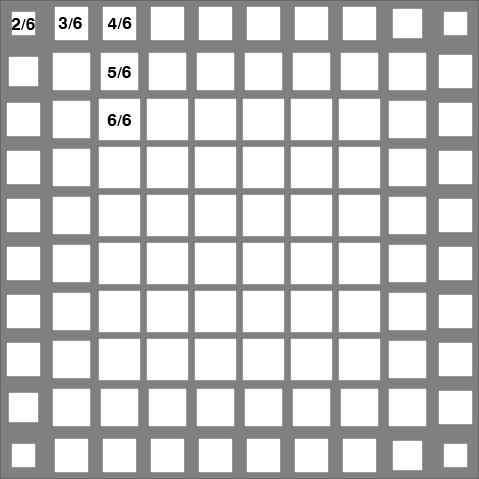
\includegraphics[width=7.8cm]{images/battleship_board_3_init_annotated.png} 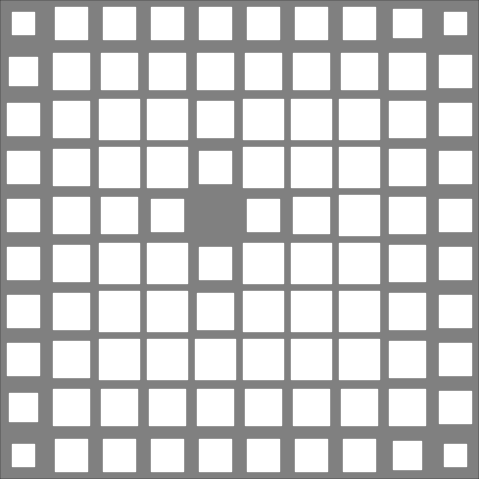
\includegraphics[width=7.8cm]{images/battleship_board_3_1miss.png}
\caption{Left: visualization of probabilities for squares to contain a ship of size 3 ($P(O_{i,j})=true$) initially, assuming uniform distribution of this type of ship. Annotations correspond to the \textit{number of combinations} (on six, the maximum number of conformations), Right: same probability after a miss in (5, 5). The larger the white area the higher the probability.}
\label{fig:battleship}
\end{center}
\end{figure}


\subsection{Poker}

%\section{Card Games}
\citep{gunn}

%%%%%%%%%%%%%%%%%%%%%%%%%%%%%%%%%%%%%%%%%%%%%%%%%%%%%%%%%%%%%%%%%% 

\section{FPS}
\subsection{Gameplay}
\subsection{FPS AI}
\subsubsection{Industry}
\subsubsection{Research}
\begin{itemize}
\item Quake 3 AI (industry standard w/o squad AI) \citep{waveren-02-artificial}
\item Killzone 2, F.E.A.R \citep{orkinGDC_FEAR} (planning), Crysis 2, BF3: industry standards with squad AI
\item Research:
\begin{itemize}
\item \citep{lehy04}
\item \citep{Laird01} (cognitive architecture)
\item others (\citep{Hladky_anevaluation} ANN, ...)
\item UT Challenge (c.f. CIG)
\end{itemize}
\end{itemize}
\subsubsection{Challenges}

%%%%%%%%%%%%%%%%%%%%%%%%%%%%%%%%%%%%%%%%%%%%%%%%%%%%%%%%%%%%%%%%%% 

\section{(MMO)RPG}

\subsection{Gameplay}
\subsection{RPG AI}
\subsubsection{Industry}
\subsubsection{Research}
\citep{Cutumisu09}
\subsubsection{Challenges}
\citep{SYNNAEVE:MMORPG}


%%%%%%%%%%%%%%%%%%%%%%%%%%%%%%%%%%%%%%%%%%%%%%%%%%%%%%%%%%%%%%%%%% 

\section{RTS}

\subsection{Gameplay}
XXX 

In chronological order, RTS include (but are not limited to): Ancient Art of War, Herzog Zwei, Dune II, Warcraft, Command \& Conquer, Warcraft II, Command \& Conquer: Red Alert, Total Annihilation, Age of Empires, StarCraft, Age of Empires II, Tzar, Cossacks, Homeworld, Battle Realms, Ground Control, Spring Engine: Balanced Annihilation, Warcraft III, Total War, Warhammer 40k, Sins of a Solar Empire, Supreme Commander, StarCraft II.

Both \citep{Human-LevelAIKillerApplication} and \cite{gunn} propose that RTS AI is one of the most challenging genres, because all levels in the hierarchy of decisions are of importance.

\subsection{RTS AI}
\subsubsection{Industry}
\subsubsection{Research}
\subsubsection{Challenges}

%%%%%%%%%%%%%%%%%%%%%%%%%%%%%%%%%%%%%%%%%%%%%%%%%%%%%%%%%%%%%%%%%% 

\section{Game Characteristics}

For a complementary taxonomy of video games and AI, see \cite{gunn}.
\subsection{Combinatory}
\subsection{Partial information}
%%%\subsection{Multiplayer}
%%%\subsection{PvE}
\subsection{Randomness}
\subsection{Time Constant(s)}
\subsection{Learning Curve}
\subsection{Recap}
\begin{sidewaystable}
\begin{tabular}{|l|ccccc|}
\hline 
Game & Combinatory & Vertical cont. & Horizontal cont. & Partial Info. & Randomness \\
\hline
Checkers & $b\approxeq 10; n\approxeq 70$ & none & none & no & no \\
Chess & $b\approxeq 40; n\approxeq 80$ & none & none & no & no \\
Go & $b\approxeq 300; n\approxeq 150$ & none & some & no & no \\
%Monopoly 
%Battleship
Limit Poker & $b\approxeq 3$\footnote{fold,check,raise} $;n/hour \in [20\dots240]$\footnote{number of decisions taken per hour} & some & few & much & much \\
Time Racing & & & & & \\
(TrackMania) & $b\approxeq 50-1,000$\footnote{$\{X \times Y\}$ sampling$\times$50Hz}$;n/min \approxeq 60$ & full & much & no & no \\
Team FPS & $b\approxeq 100-5,000$\footnote{\label{samplingFPS}$\{X \times Y \times Z\}$ sampling$\times$50Hz + firing} $;n/min \approxeq 100$\footnote{\label{apmFPS}60 ``continuous move actions''+ 40 (mean) fire actions per sec} & some & much & some & some \\
(Counter-Strike) & & & & & \\
(Team Fortress 2) & & & & & \\
FFPS duel & $b\approxeq 200-10,000$\footref{samplingFPS} $;n/min \approxeq 100$\footref{apmFPS} & some & much & some & ($\approxeq$)no \\
(Quake III) & & & & & \\
MMORPG & $b\approxeq 50-100$\footnote{in RPGs, the player does not have to aim and positioning plays a lesser role than in FPS} $;n/min \approxeq 60$\footnote{move and use abilities/cast spells} & much & much & few & moderate \\
(WoW, DAoC) & & & & & \\
RTS & $b\approxeq 200$\footnote{atomic dir/unit $\times$ \# units + constructions + productions}$;n/min=APM\approxeq 300$\footnote{for progamers, counting group actions as only one action}& some & some & much & no\\
(StarCraft) & & & & & \\
\hline
\end{tabular}
\end{sidewaystable}

%%%%%%%%%%%%%%%%%%%%%%%%%%%%%%%%%%%%%%%%%%%%%%%%%%%%%%%%%%%%%%%%%% 

\section{Player Characteristics}

%%% Timings, reflexes, modeling, goals, utility, backtracking, induction, ...

In all these games, knowledge and learning plays a key role. Humans compensate their lack of (conscious) computational power with pattern matching, abstract thinking and efficient memory structures. 
\subsection{Virtuosity}
Skill
\subsection{Deduction}
\subsection{Induction}
\subsection{Decision-Making}
%%%\subsection{Psychology}
\subsection{Recap}
%%% https://en.wikipedia.org/wiki/Cognition
\begin{sidewaystable}
\begin{tabular}{|l|ccccccc|}
\hline 
Game & Virtuosity & Deduction & Induction & Decision-Making & \multicolumn{3}{c|}{Knowledge} \\
     & (sensory-motor) & (analysis) & (abstraction) & (acting) & game & map & opponent \\
Checkers &   & ++ & &   & ++& &+ \\
Chess &   & ++ & &   & ++& &+ \\
Go &   & ++ & + &   & ++& &+ \\
Limit Poker &   & + & + & ++ & ++& &++ \\
Time Racing & ++ &   &   &   & +&++&  \\
(TrackMania) & & & & & & & \\
Team FPS & & & & & & & \\ 
(Counter-Strike) & & & & & & & \\ 
(Team Fortress 2) & & & & & & & \\ 
FFPS duel & ++ & + &   & + & +&++&+ \\
(Quake III) & & & & & & & \\ 
MMORPG & + & + & + & ++ & +&++&+ \\
(WoW, DAoC) & & & & & & & \\ 
RTS & ++ & ++ & ++ & ++ & ++&+&++ \\
(StarCraft) & & & & & & & \\
\hline
\end{tabular}
\end{sidewaystable}

%%%%%%%%%%%%%%%%%%%%%%%%%%%%%%%%%%%%%%%%%%%%%%%%%%%%%%%%%%%%%%%%%% 

\section{An interesting problem}
\subsection{Simulated but stochastic}
Human players (ally or foes), and sometimes (most of the time) stochasticity in the rules of the game (fog of war, randomness, etc.).
